\section{The Model} \label{sec:the_model}

Our modeling efforts are divided into two main levels: macro and micro. Our micro model, a discrete cellular automata model inspired by \cite{Nagel1992ATraffic}, predicts the relationship between traffic density and traffic speed. This model is used to predict how this relationship between traffic density and flow rate will change with different concentrations of self-driving vehicles on the road. Our macro model, a system of ordinary differential equations, considers how the relationship between traffic density and traffic speed will affect regional traffic patterns in the Puget Sound area. This model ultimately makes predictions about expected travel time between regional destinations of interest.

\subsection{Micro/Discrete Model}

To see how the fundamental diagram changes as the number of self-driving cars increases, we set up a cellular automata model based on work by Nagel and Schrekenberg. In their original model, each car follows three rules at each time-step However, to model the effects of self-driving cars, we used the following modified rules.
\begin{enumerate}
	\item \textbf{Acceleration}: The $i$th car moving with velocity $v_i$ will increase its velocity by 1 so long as the car ahead is greater than $v_i+g$ or $v_i+g$ units away, where $g=2$ for a human driver, and $1$ for self-driven car.
    \item \textbf{Slowing down}: If the car ahead is instead $j$ units away with $j\leq v_i$, the velocity will decrease to $j-g$ or 0 if $j-g<0$.
    \item \textbf{Randomization}: Every car has a probability $p$ of randomly decreasing their velocity by 1. For human-driven cars $p=0.1$, and for self-driven cars, $p_s=0.05$.
\end{enumerate}
Once the velocities for every car is updated, each car is then moved ahead by $v_i$ units. The density was calculated by counting the number of times a car lands on the center cell of the track, while the flux is calculated by counting the number of times a car passes through the center cell.

\subsection{Using the Micro Model to Inform the Macro Model}
Having developed a micro model, we need to extract useful density and velocity information to run the macro model.  We do this by fitting our data from the micro model to a simplification of the curve shown in Figure \ref{fig:micro-schematic}, which we have adapted from \cite{Dym2004PrinciplesModeling}.  The curious reader can find a more in-depth explanation of this fit in Dym's text.  Our micro model data fits the red curve; however, for the sake of more efficient computation, we have chosen to apply a linear fit between the points ($\rho_{crit}$,$v_{max}$) and ($\rho_{max}$, 0). This linear fit was inspired by Greenshield's model of the relationship between traffic flow and traffic speed \cite{KachrooTrafficFramework}. Using this fit, we can determine the relationship between traffic density ($\rho$) and flow speed ($v$) in our macro model.

\begin{figure}[h]
\centering
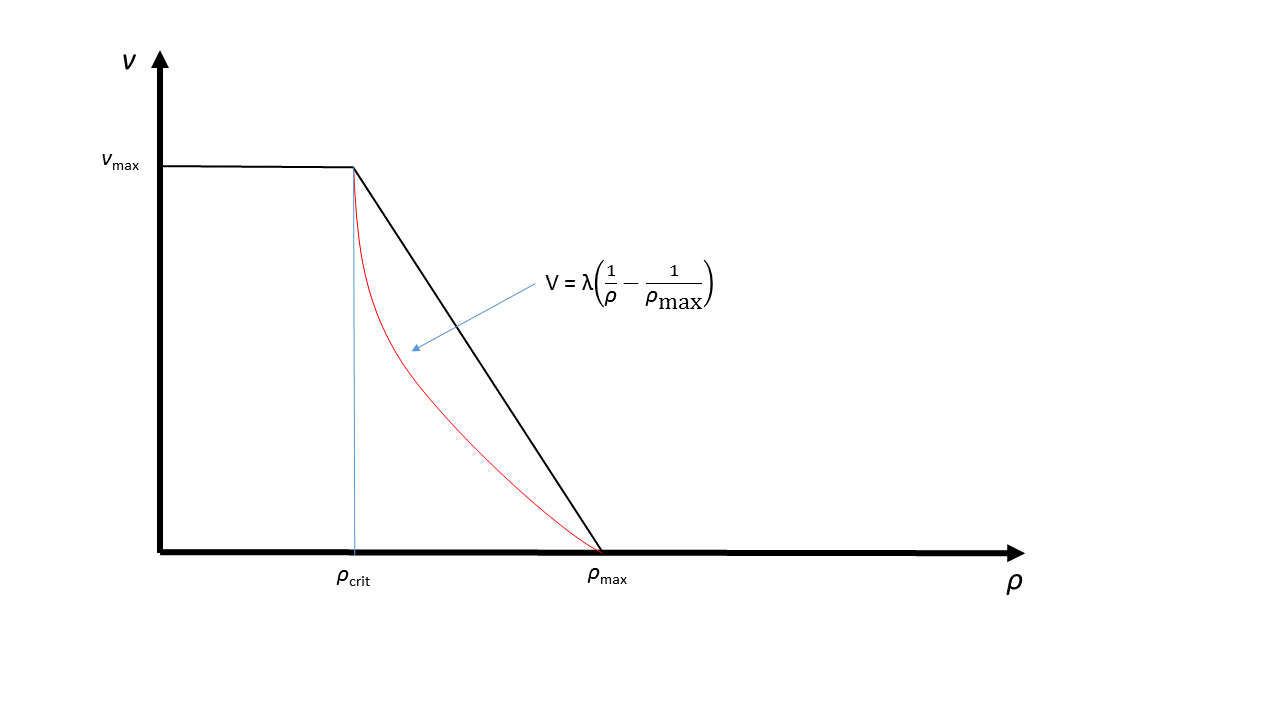
\includegraphics[width=0.9\textwidth]{img/micro-schematic.png}\\
\caption{Original (in red, from \cite{Dym2004PrinciplesModeling}) and simplified flux curves illustrating speed-density relationship.}
\label{fig:micro-schematic}
\end{figure}

Our micro model predicts the following $\rho_{crit}$ values for differing proportions of self-driving traffic. (Note that no significant difference in $\rho_{crit}$ was observed between 0\% self-driving traffic and 10\% self-driving traffic.)

\bigskip

\begin{tabular}{
|p{2cm}|p{2cm}|p{2cm}| }
 \hline
 \multicolumn{3}{|c|}{$\rho_{crit}$ versus self-driving traffic proportion} \\
 \hline
 0-10\% & 50\% & 90\% \\
 \hline
  0.13 & 0.16 & 0.18 \\
 \hline
\end{tabular}

\subsection{Macro/Continuous Model}

Our model, at the most fundamental level, traces the evolution of the number of cars on the road.  Before further developing our simulation, we must establish the following useful quantities for the $i$th road segment. 

\begin{align}
L_i = D_i \times N_{Li}
\end{align}

gives the ``lane length" of the road.  This essentially allows cars to distribute evenly across the number of lanes available on road segment $i$.  We next calculate car density,

\begin{align}
\rho_i = \frac{N_i}{L_i} 
\end{align}

which we will use in computing the net car flux through the $i$th road segment, given as developed by Fowkes and Mahony in their text, \textit{An Introduction to Mathematical Modeling}, to be

\begin{align}
F_i = \rho_i \times V_i
\end{align}

We begin with a first-order differential equation for the rate of change in time of the total number of cars on the $i$th road segment. We assume that cars flow into each segment at the road-length density of traffic in the preceding segment and the  velocity of cars at that segment. We assume that cars flow out of each segment at the road-length density of traffic in that segment and the velocity of cars at the next segment. For a visualization of an arbitrary internal road segment, see Figure \ref{fig:ODE-schematic}. Additionally, we assume that cars enter or exit the segment at a constant rate determined by the difference in average traffic between the previous segment and the current segment. This gives the relationship:

\begin{align}
\frac{dN_i}{dt} = v_{i} \times \rho_{i-1} - V_{i+1} \times \rho_{i} + \Delta C_i - \Delta C_{i + 1}
\end{align}

\begin{figure}[h]
\centering
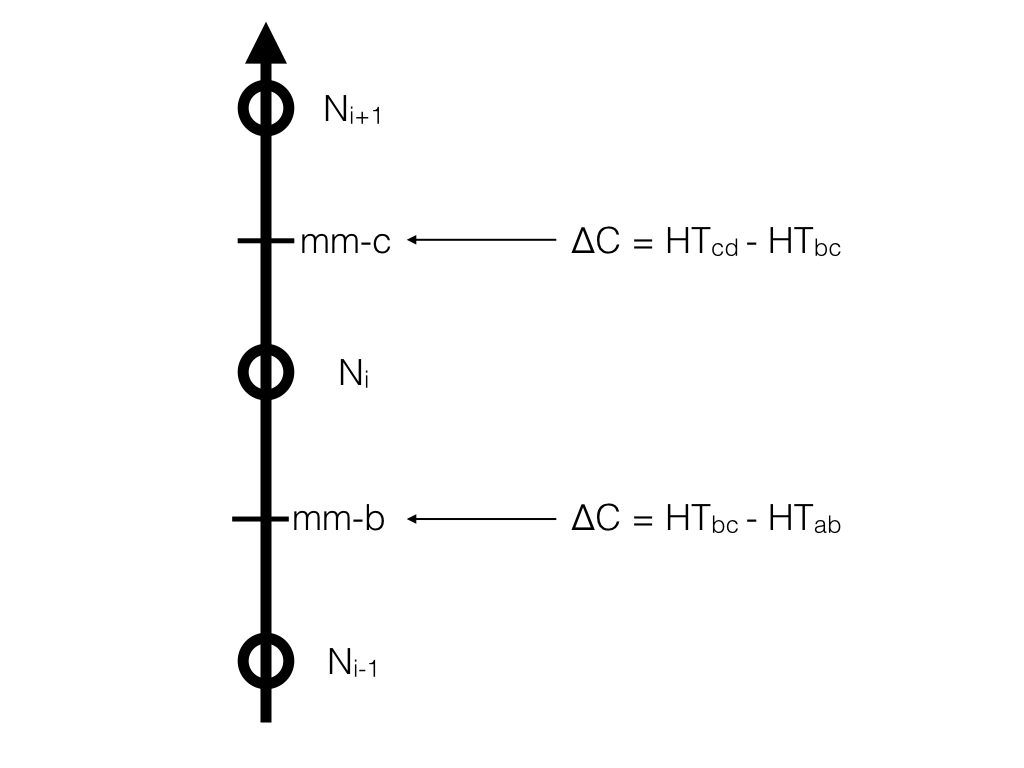
\includegraphics[width=0.7\textwidth]{img/macro-traffic.png}\\
\caption{Schematic of $i$th road segment as a circular node.  Here mm-x refers to mile-marker x, and $\Delta C$ keeps track of the cars that have entered or exited the road between nodes.}
\label{fig:ODE-schematic}
\end{figure}

We model each direction of travel on each highway as a separate one-dimensional chain of highway segments. We do not model intersections between highways. For each highway system road segment at the beginning of a highway chain, we model cars as entering at a fixed rate $C$ determined by the AADT recorded for the road segment. For each highway system road segment at the end of a highway chain, we model cars as leaving with traffic speed 50 miles per hour at the current traffic density of the end segment. This approach yields several systems of ordinary differential equations, which can be evaluated numerically. We use the Numpy \texttt{odeint} tool for this purpose \cite{Jones2001SciPy:Python}. 

We determine the traffic speed $V$ at each segment from its density $\rho$ using a smooth interpolation using B-splines of the density-flow rate predictions made by the discrete traffic flow model. To run the regional traffic model at peak traffic conditions, we simply scale the net traffic load uniformly across the system by $1.92$, reflecting the observation that peak traffic volume observed over the course of an hour represents $8\%$ of ADT on that segment.
\begin{align*}
T_{peak} / 24 = 0.08 \times T_{avg} \\
T_{peak}  = 24 \times 0.08  T_{avg} = 1.92 \times  T_{avg}   \\
\end{align*}
ADT for each direction of each segment is one-half ADT reported for each segment, reflecting the assumption that traffic load at each segment is split evenly between the increasing and decreasing directions.

We run the simulation, beginning with initial conditions of a uniform distribution of traffic between road segments at a density of 25 cars per lane-mile, until it reaches a near-equilibrium state. Then, the density of traffic on each road segment is recorded. (For reported simulations, data on traffic density was collected after five hours of simulation time). This density information, coupled with the relationship between traffic density and traffic speed predicted by the micro model, yields travel time $t$ between road segments $i$ and $j$ according to the following relationship
\begin{align*}
t = \sum_{n = i}^{j} \frac{D_n}{V(\rho_n)}
\end{align*}

\subsection{Micro/Discrete Model Validation}
The results from the discrete model closely resembles results found in all of the literature we observed\cite{KachrooTrafficFramework,Dym2004PrinciplesModeling}. Specifically, we looked to reproduce results from Nagel and Schrekenberg\cite{Nagel1992ATraffic} as a starting point for modeling the effects of self-driving cars. We were also able to very closely fit our results to a model in Dym \cite{Dym2004PrinciplesModeling}. 
\subsection{Macro/Continuous Model Validation} \label{sec:macro_validation}

We validated our traffic model by comparing trip times for northbound and southbound traffic on popular stretches of roads to actual traffic data from the WSDOT website \cite{WSDOT2017WSDOTTimes}. Specifically, we compared our model's predictions for travel times between a representative sampling of destinations of interest under average traffic conditions to WSDOT travel time data for non-peak traffic conditions. Our model made reasonable predictions under these conditions, often with error mostly below 20\%. However, the macro model fares much more poorly at higher traffic levels, exhibiting significant error. Traffic jams -- apparent through significantly lengthened travel time between destinations -- do not manifest until quantitative traffic loads much beyond the traffic levels observed at peak traffic hours. At traffic loads approximately 50\% greater than observed peak traffic and above, significant delays are observed on some highways, in particular I-5 South and I-405. This inconsistency may be due to the decision to model high-load traffic a static elevated demand upon highway infrastructure instead of a process where demand grows, peaks, and declines over time. Optimistic boundary conditions, which assume that traffic leaves the system mostly unimpeded may also contribute to the excess optimism of the model. Discrepancies in the translation of traffic flow predictions from the micro model to the macro model -- such as the limited fidelity of the Greenshield-like linear fit to the micro model's predictions or distorted unitary scale in analysis of the micro model's predictions may also account for the discrepancy. Also, the neglect of traffic-blocking incidents such as breakdowns and accidents may why our traffic predictions are not as dire as WSDOT's 95\% Worst Case Scenario travel times. Although further refinement this macro model is necessary for it to have quantitative relevance, we believe that it does have qualitative value in understanding the impact of the introduction of self-driving cars on Seattle traffic. Observed model predictions on travel times are tabulated below beside relevant reported WSDOT data.

\vspace{12pt}

\noindent \begin{tabular}{
|p{1.5cm}|p{1.5cm}||p{1cm}|p{1.5cm}|p{1.5cm}|p{1.5cm}|p{2cm}|p{1cm}|  }
 \hline
 \multicolumn{7}{|c|}{Average Trip Times on Key Routes (Increasing/Decreasing)} \\
 \hline
 Origin & Dest & Road ID& Distance (miles) & Avg. Travel Data (min) & Avg. Travel Model (min) & \% Error \\
 \hline
 Fed. Way    & Seattle  & 5  & 22.2 & 22 & 22.6 & 3 \\
 Seattle     & Everett  & 5  & 26.9 & 27 & 29.4 & 9 \\
 Seattle     & Issaquah & 90  & 15.7 & 16 & 14.9 & 7 \\
 Bellvue     & Redmond  & 520 & 6.6  & 7  & 5.9 &  16 \\
 Renton      & Bellvue  & 405 & 11.2  & 11 & 11.1 & 1 \\
 Seattle  & Fed. Way  & 5  & 22.2 & 24 & 22.6 & 6 \\
 Everett  & Seattle  & 5   & 26.9 & 27 & 29.4 & 9 \\
 Issaquah & Seattle & 90  & 15.7 & 17 & 14.9 & 12 \\
 Redmond  & Bellvue  & 520 & 6.6  & 8  & 5.9 & 26 \\
 Bellvue  & Renton  & 405 & 11.2  & 11 & 11.1 & 1 \\
 \hline
\end{tabular}
\\
\bigskip
\\
\noindent \begin{tabular}{
|p{1.5cm}|p{1.5cm}||p{0.75cm}|p{1.25cm}|p{2.5cm}|p{2cm}|p{1.5cm}|p{1.5cm}|p{1.5cm}| }
 \hline
 \multicolumn{9}{|c|}{Peak Trip Times on Key Routes (Increasing/Decreasing)} \\
 \hline
 Origin & Dest & Road ID& Distance (miles) & 8:00 am Worst-Case Travel Data (min) & 8:00 am Peak Travel Model (min) & \% Error Peak Travel Model  &  1.6$\times$ Peak Travel Model &  \% Error 1.6$\times$ Peak Travel Model \\
 \hline
 Fed. Way    & Seattle  & 5   & 22.2 & 69 & 22.7 & 67 & 25.1 & 64 \\
 Seattle     & Everett  & 5   & 26.9 & 28 & 29.8 & 6 & 34.1 & 22 \\
 Seattle     & Issaquah & 90  & 15.7 & 22 & 14.9 & 32 & 15.7 & 29 \\
 Bellvue     & Redmond  & 520 & 6.6  & 8  & 5.9 & 26 & 6.4 & 20 \\
 Renton      & Bellvue  & 405 & 11.2  & 51 & 11.8 & 77 & 18.0 & 64 \\
 Seattle  & Fed. Way  & 5   & 22.15 & 25 & 14.9 & 40 & 25.4 & 2 \\
 Everett  & Seattle  & 5   & 26.94 & 89 & 30.0 & 66 & 76.8 & 14 \\
 Issaquah & Seattle & 90  & 15.71 & 36 & 14.3 & 60 & 15.7 & 56 \\
 Redmond  & Bellvue  & 520 & 6.62 & 11 & 5.9 & 46 & 6.4 & 42 \\
 Bellvue  & Renton  & 405 & 11.2  & 27 & 11.8 & 56 & 19.3 & 28 \\
 \hline
\end{tabular}
